\documentclass[10pt,twocolumn]{article}
% Packages
\usepackage{times}
\usepackage[fleqn]{amsmath}
\usepackage{amssymb}
\usepackage{anysize}
\usepackage{multicol}
\usepackage{graphicx}
\usepackage{booktabs}
\usepackage{titlesec}
\usepackage{float}
\usepackage{natbib}
%\restylefloat{table}
\usepackage[tableposition=top]{caption}
% Options
\marginsize{2.5cm}{1.5cm}{1cm}{1cm}
\setlength{\columnsep}{18.0pt}
% Title spec
\title{COMP3130 -- Group Project in Computer Science\\ Warm-up Project -- 4$\times$4$\times$4 TicTacToe Agent}
\date{March 24, 2012}
\author{Andrew Haigh -- u4667010;\\ Timothy Cosgrove -- u4843619;\\ Joshua Nelson -- u4850020}
% Section styling
\titleformat{\section}%
  {\large\itshape}%
  {\thesection.}{.5em}{}%
  [\vspace{1ex}\titlerule]%
\titleformat{\subsection}%
  {\itshape}%
  {\thesubsection.}{.5em}{}%
\begin{document}
\onecolumn
\maketitle
\twocolumn
\section{Abstract}
The purpose of this project was to implement an intelligent agent to play 3
dimensional 4 by 4 by 4 Tic Tac Toe. We chose to implement this in C, with a
pipe interface to python. This allowed us to use python's 3D libraries for visualisation
while utilising the speed of a compiled C program.

\section{Solution Overview}
The core of the agent is implemented with a combination of minimax and $\alpha$-$\beta$ pruning.

Board states are stored simply as a 3 dimensional array of chars; but this data is passed
through the program as a struct including extra information such as a heuristic evaluation
of the state. Once the minimax program reaches a fixed cut-off depth we select a state based on
this heuristic. For testing purposes all code is compiled with the -g flag. This allows
us to use the program \texttt{gprof} to analyse running time and total number of function calls
(this is used to optimise and evaluate the effectiveness of $\alpha$-$\beta$ pruning).

\subsection{Overview of modules}
\texttt{visualisation.py:}
\begin{itemize}
\item The python module which takes user input and displays the game board using VPython
\item This is the main program, it creates a sub-process (\texttt{worker.c}) which returns
board states to display
\item Contains several visualisation options: press 'g' to switch views and 's' to enable
red-cyan stereoscopic 3D.
\end{itemize}
\begin{figure}[h]
  \begin{center}
    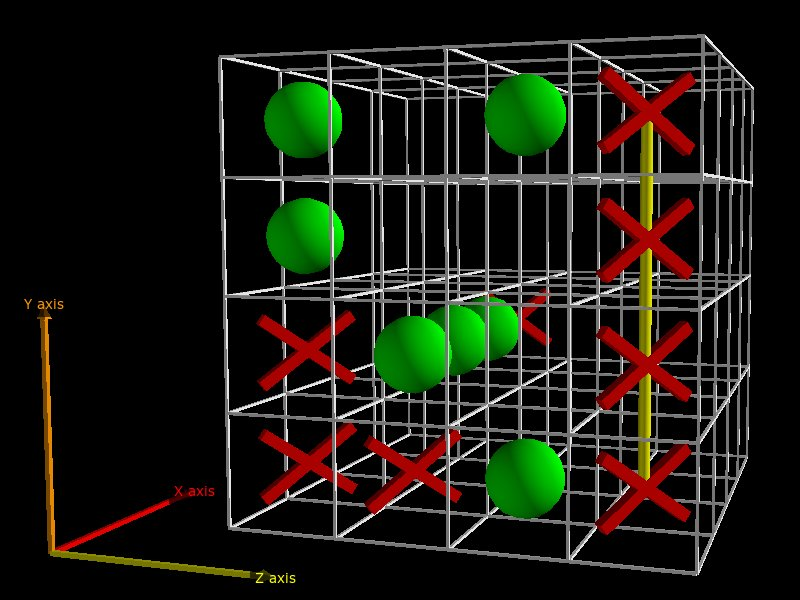
\includegraphics[width=2in]{vis.jpg}
  \end{center}
  \caption{Example of a game visualisation}
  \label{fig:vis}
\end{figure}
\texttt{worker.c:}
\begin{itemize}
\item The link module which handles communication between python and C
\item Calls code from \texttt{state\_functions.c} to start minimax and pick the next move
\end{itemize}
\texttt{state\_functions.c:}
\begin{itemize}
\item Contains all core functionality of the AI agent including minimax functions and state
evaluation functions
\item Includes a simple victory function which checks if a player has won with a line nearby to
the most recent move. (comprehensive victory checks are made in \texttt{visualisation.py})
\end{itemize}

\section{State Space for 4$\times$4$\times$4}
In the original scope of this project we had intended to examine the entire state space
before making a move. However, the state space is in fact exceedingly large. Considering all
possible states we have $3^{64}$, but many of these (far more than half) are illegal or unreachable.
According to \cite{Patashnik1980}, after 18 moves (under perfect play by player 1)
the game will be over or in a state where every move is forced. With this in mind we can 
consider a more reasonable upper bound on the states we must examine:
 \[\binom{64}{18} = 3601688791018080\]
If we assume we can examine 1 state per clock cycle (a completely and utterly unreasonable assumption) it would
still take 250 hours to search this reduced state space on a 4GHz CPU. Minimax with $\alpha$-$\beta$ pruning
and other clever tricks could significantly reduce this figure; however it remains obvious that
searching to depth 18 for every move is unachievable. Thus we set a depth cut-off where we stop
searching and perform a heuristic state evaluation.

Due to this inevitable cut-off it also became impossible to determine if either
player has a winning strategy. It is however interesting to note that (in the paper
mentioned above) Patashnik determined that the first player can always win with perfect play. 

\section{Heuristics and Cut-offs}
briefly explain heuristics and cut off decisions



\section{Pure minimax vs.\ $\alpha$-$\beta$ pruning}
Some tests were run using the Unix tool \texttt{gprof} to determine the effectiveness
of heuristics and $\alpha$-$\beta$ pruning. By counting the number of calls
to our state-evaluation function we get the total number of examined leaf nodes.
Furthermore \texttt{gprof} returns a summary of how much time (in seconds) is spent running
each function and the whole program.

The tables below summarise \texttt{gprof} results when the agent is making it's first move;
run at various cut-off depths:
\begin{table}[H]
  \centering
  \caption{Total leaf nodes examined}
  \begin{tabular}{lrrr}
    \toprule
    Depth & Minimax & $\alpha$-$\beta$ & $\alpha$-$\beta$ + Heuristics \\
    \midrule
    3 & 249984 & 8026 & ??? \\
    4 & 15249024 & 256936 & ??? \\
    5 & 914941440 & 622961 & ??? \\
    6 & 53981544960 & 16771844 & ??? \\
    7 & <++> & <++> & ??? \\
    \bottomrule
  \end{tabular}
  \label{tab:leafnodes}
\end{table}
\begin{table}[h]
  \centering
  \caption{Total time taken (seconds)}
  \begin{tabular}{lccc}
    \toprule
    Depth & Minimax & $\alpha$-$\beta$ & $\alpha$-$\beta$ + Heuristics \\
    \midrule
    3 & 0.27 & 0.03 & ??? \\
    4 & 15.30 & 0.24 & ??? \\
    5 & 941.99 & 1.18 & ??? \\
    6 & ??? & ??? & ??? \\
    7 & ??? & 116.77 & ??? \\
    \bottomrule
  \end{tabular}
  \label{tab:time}
\end{table}

The benefits of $\alpha$-$\beta$ pruning are obvious and indisputable, often cutting
the number of nodes and total time by a factor of over 1500.
However, the benefits of our heuristic function are less obvious. We notice that
a great deal less leaf nodes are examined; but the improvement in running time is
negligible. This is due to the fact that we must constantly evaluate states for their
potential value; taking precious CPU time.

\section{Summary and Reflection}
A Summary. Also discuss how this will prepare us for reversi (language choice,
teamwork, gitHub)

\bibliographystyle{alpha}
\bibliography{ai}
\end{document}
